%%
%% This is file `tikzposter-template.tex',
%% generated with the docstrip utility.
%%
%% The original source files were:
%%
%% tikzposter.dtx  (with options: `tikzposter-template.tex')
%%
%% This is a generated file.
%%
%% Copyright (C) 2014 by Pascal Richter, Elena Botoeva, Richard Barnard, and Dirk Surmann
%%
%% This file may be distributed and/or modified under the
%% conditions of the LaTeX Project Public License, either
%% version 2.0 of this license or (at your option) any later
%% version. The latest version of this license is in:
%%
%% http://www.latex-project.org/lppl.txt
%%
%% and version 2.0 or later is part of all distributions of
%% LaTeX version 2013/12/01 or later.
%%


\documentclass{tikzposter} %Options for format can be included here

\usepackage{showframe}
\usepackage{todonotes}
\usepackage[ruled]{algorithm2e}
\usepackage[tikz]{bclogo}
\usepackage{lipsum}
\usepackage{amsmath}
\usepackage{algorithm}
\usepackage{algorithmic}
\usepackage{booktabs}
\usepackage{longtable}
\usepackage[absolute]{textpos}
\usepackage[it]{subfigure}
\usepackage{graphicx}
\usepackage{cmbright}
\usepackage{setspace}
%\usepackage[default]{cantarell}
%\usepackage{avant}
%\usepackage[math]{iwona}
\usepackage[math]{kurier}
\usepackage[T1]{fontenc}


%% add your packages here
\usepackage{hyperref}
% for random text
\usepackage{lipsum}
\usepackage[english]{babel}
\usepackage[pangram]{blindtext}
\colorlet{backgroundcolor}{blue!10}

 % Title, Author, Institute
\title{Flip 00 project final report}
\author{Jin Chen}
\institute{ HuNan University, China
}
%\titlegraphic{logos/tulip-logo.eps}

%Choose Layout
\usetheme{Wave}

%\definebackgroundstyle{samplebackgroundstyle}{
%\draw[inner sep=0pt, line width=0pt, color=red, fill=backgroundcolor!30!black]
%(bottomleft) rectangle (topright);
%}
%
%\colorlet{backgroundcolor}{blue!10}

\begin{document}


\colorlet{blocktitlebgcolor}{blue!23}

 % Title block with title, author, logo, etc.
\maketitle

\begin{columns}
 % FIRST column
\column{0.5}% Width set relative to text width

%%%%%%%%%% -------------------------------------------------------------------- %%%%%%%%%%
 %\block{Main Objectives}{
%  	      	\begin{enumerate}
%  	      	\item Formalise research problem by extending \emph{outlying aspects mining}
%  	      	\item Proposed \emph{GOAM} algorithm is to solve research problem
%  	      	\item Utilise pruning strategies to reduce time complexity
%  	      	\end{enumerate}
%%  	      \end{minipage}
%}
%%%%%%%%%% -------------------------------------------------------------------- %%%%%%%%%%


%%%%%%%%%% -------------------------------------------------------------------- %%%%%%%%%%
		\block{Introduction}{
	The data contains the location and circumstances of every field goal 
	attempted by Kobe Bryant took during his 20-year career. The task is to predict whether the basket went in (shot\_made\_flag).
	The following is the attributes list of data:
	\vspace{.5cm}
	\begin{description}
		\item[shot\_made\_flag] Yes=1,No=0
		
		\item [action\_type] \emph{Jumpshot},\emph{Layup},\emph{Dunk},
		\emph{Tipshot},\emph{Hookshot},\emph{Bankshot}
		
		\item[loc\_x ,loc\_y] shots position
		\item[shot\_type] 2PT Field Goal,2PT Field Goal
		\item[shot\_zone\_area] shots area by area
		\item[shot\_zone\_range] shots area by radius
		\item[shot\_zone\_basic] shots area by NBA rules 
		\item[shot\_made\_flag] \emph{Yes=1}, \emph{No=0}
	\end{description}
	\vspace{.3cm}
}
%%%%%%%%%% -------------------------------------------------------------------- %%%%%%%%%%


%%%%%%%%%% -------------------------------------------------------------------- %%%%%%%%%%
\block{Data Visualization}{
	The following figures show
	the distribution of the data. 
	The histogram shows the shot accuracy of various action type.
	The line chart shows the Kobe's shots positioning with distances.
	And the scatter plot shows that 
	data is distributed normally. 
	and most pairs are widely scattered  
	but some of them show clusters.


	\vspace{.5cm}
	\begin{center}
		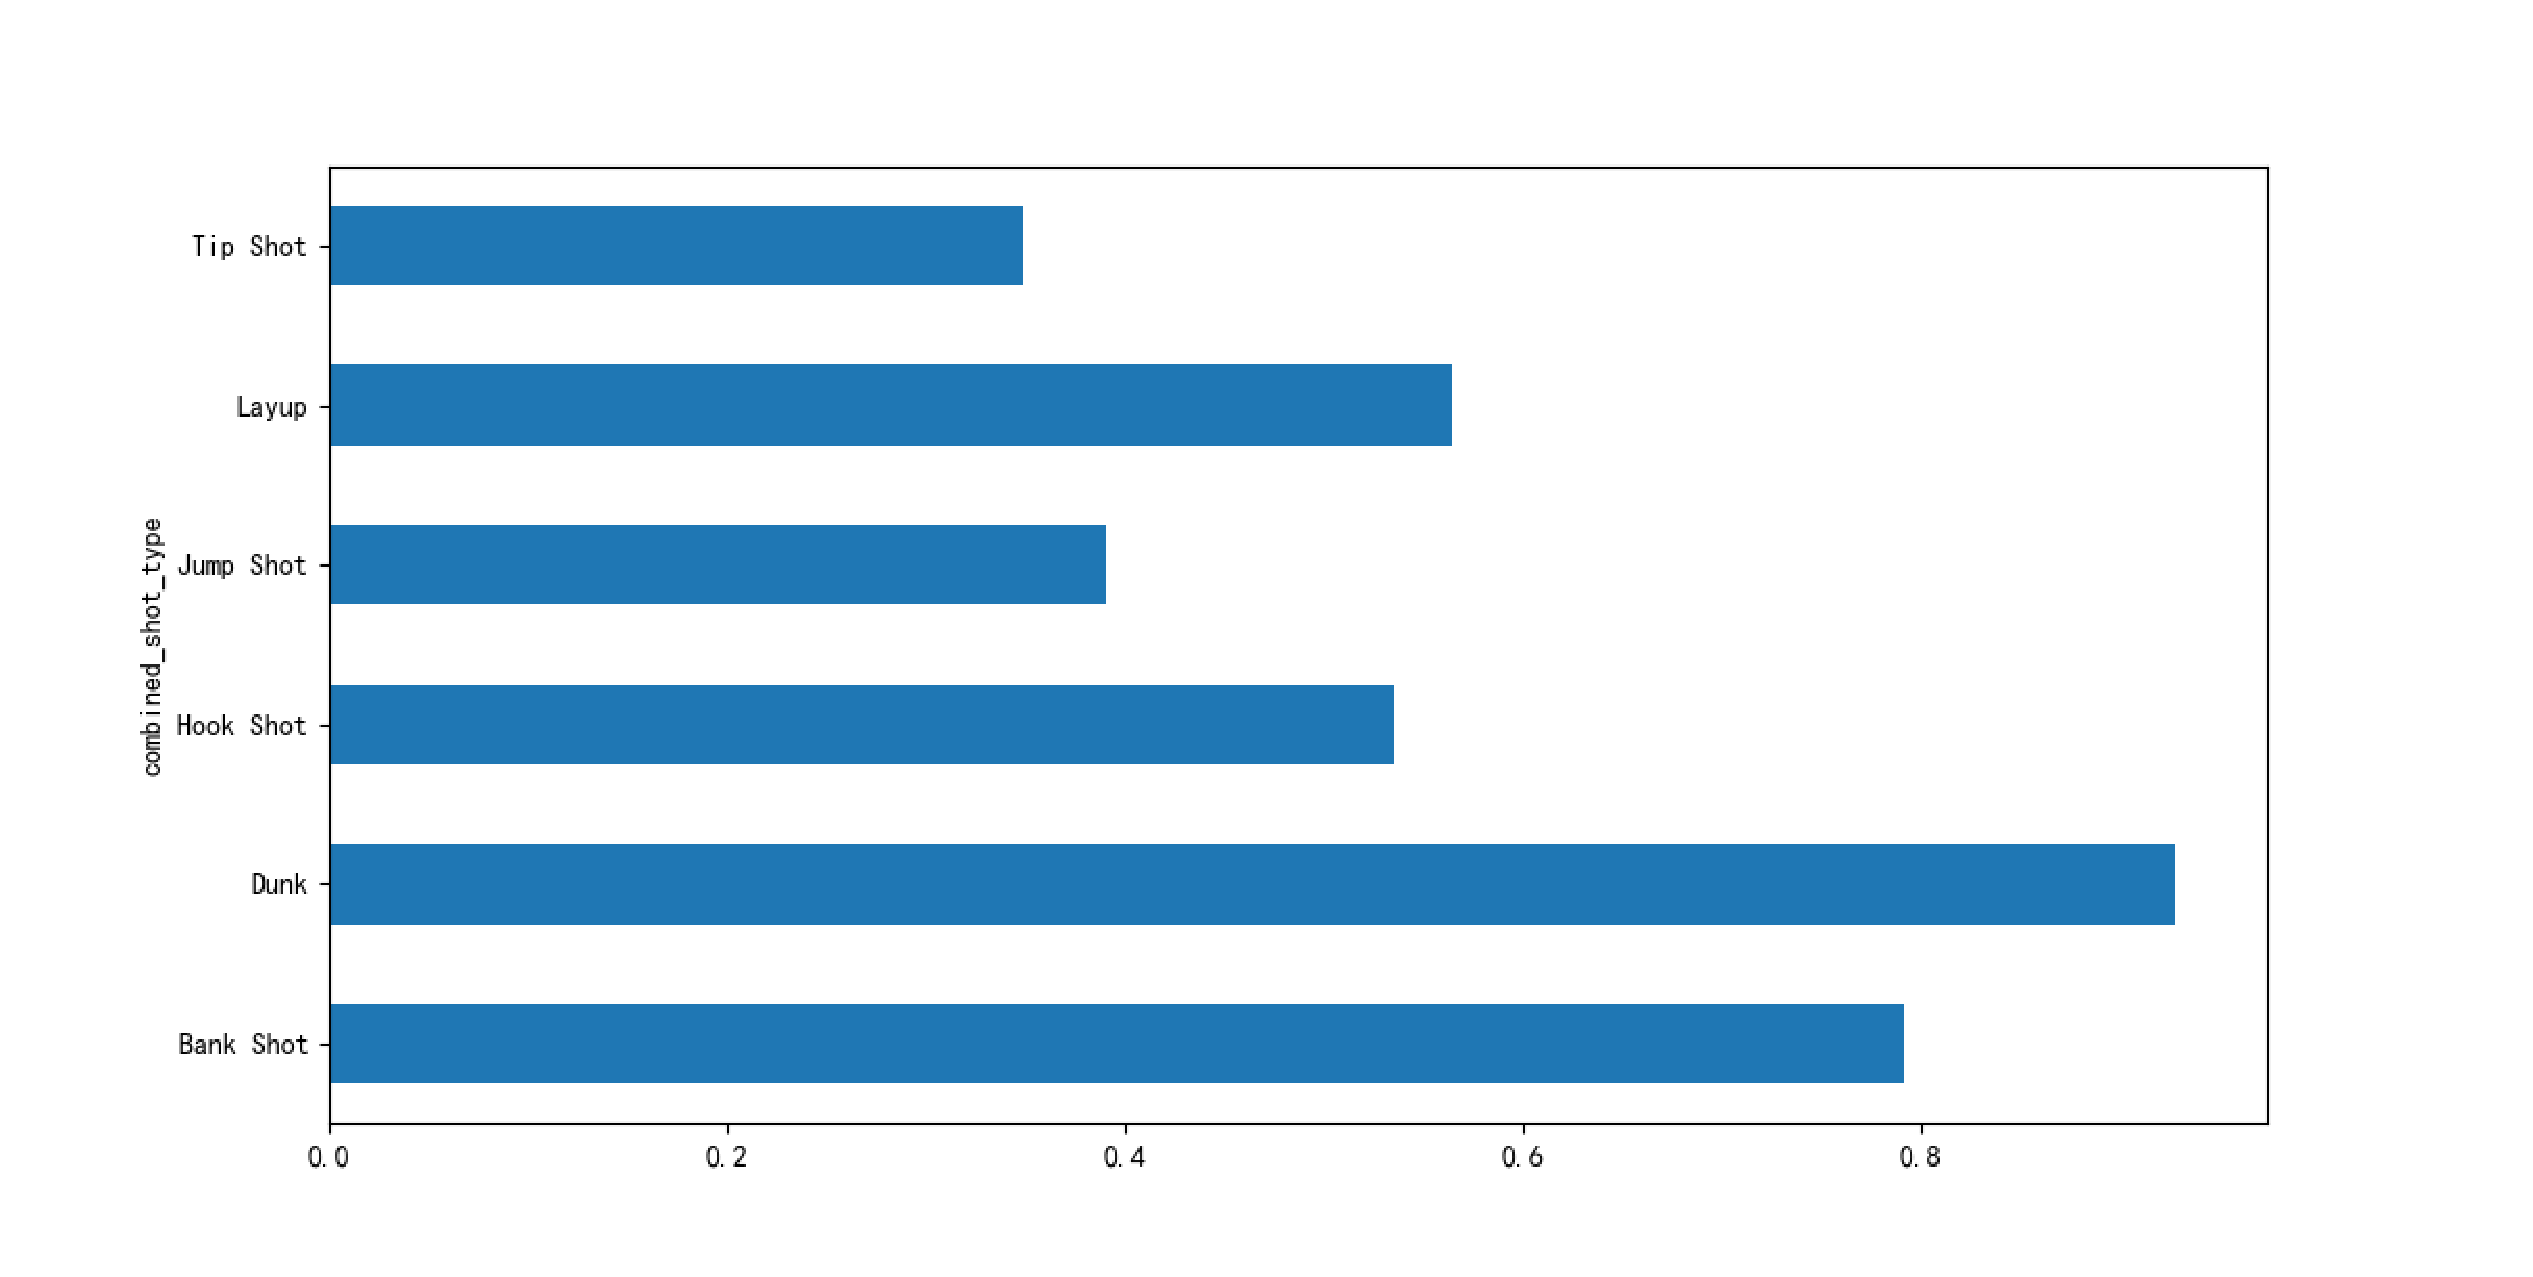
\includegraphics[width=.3\linewidth]{f.eps}
		\quad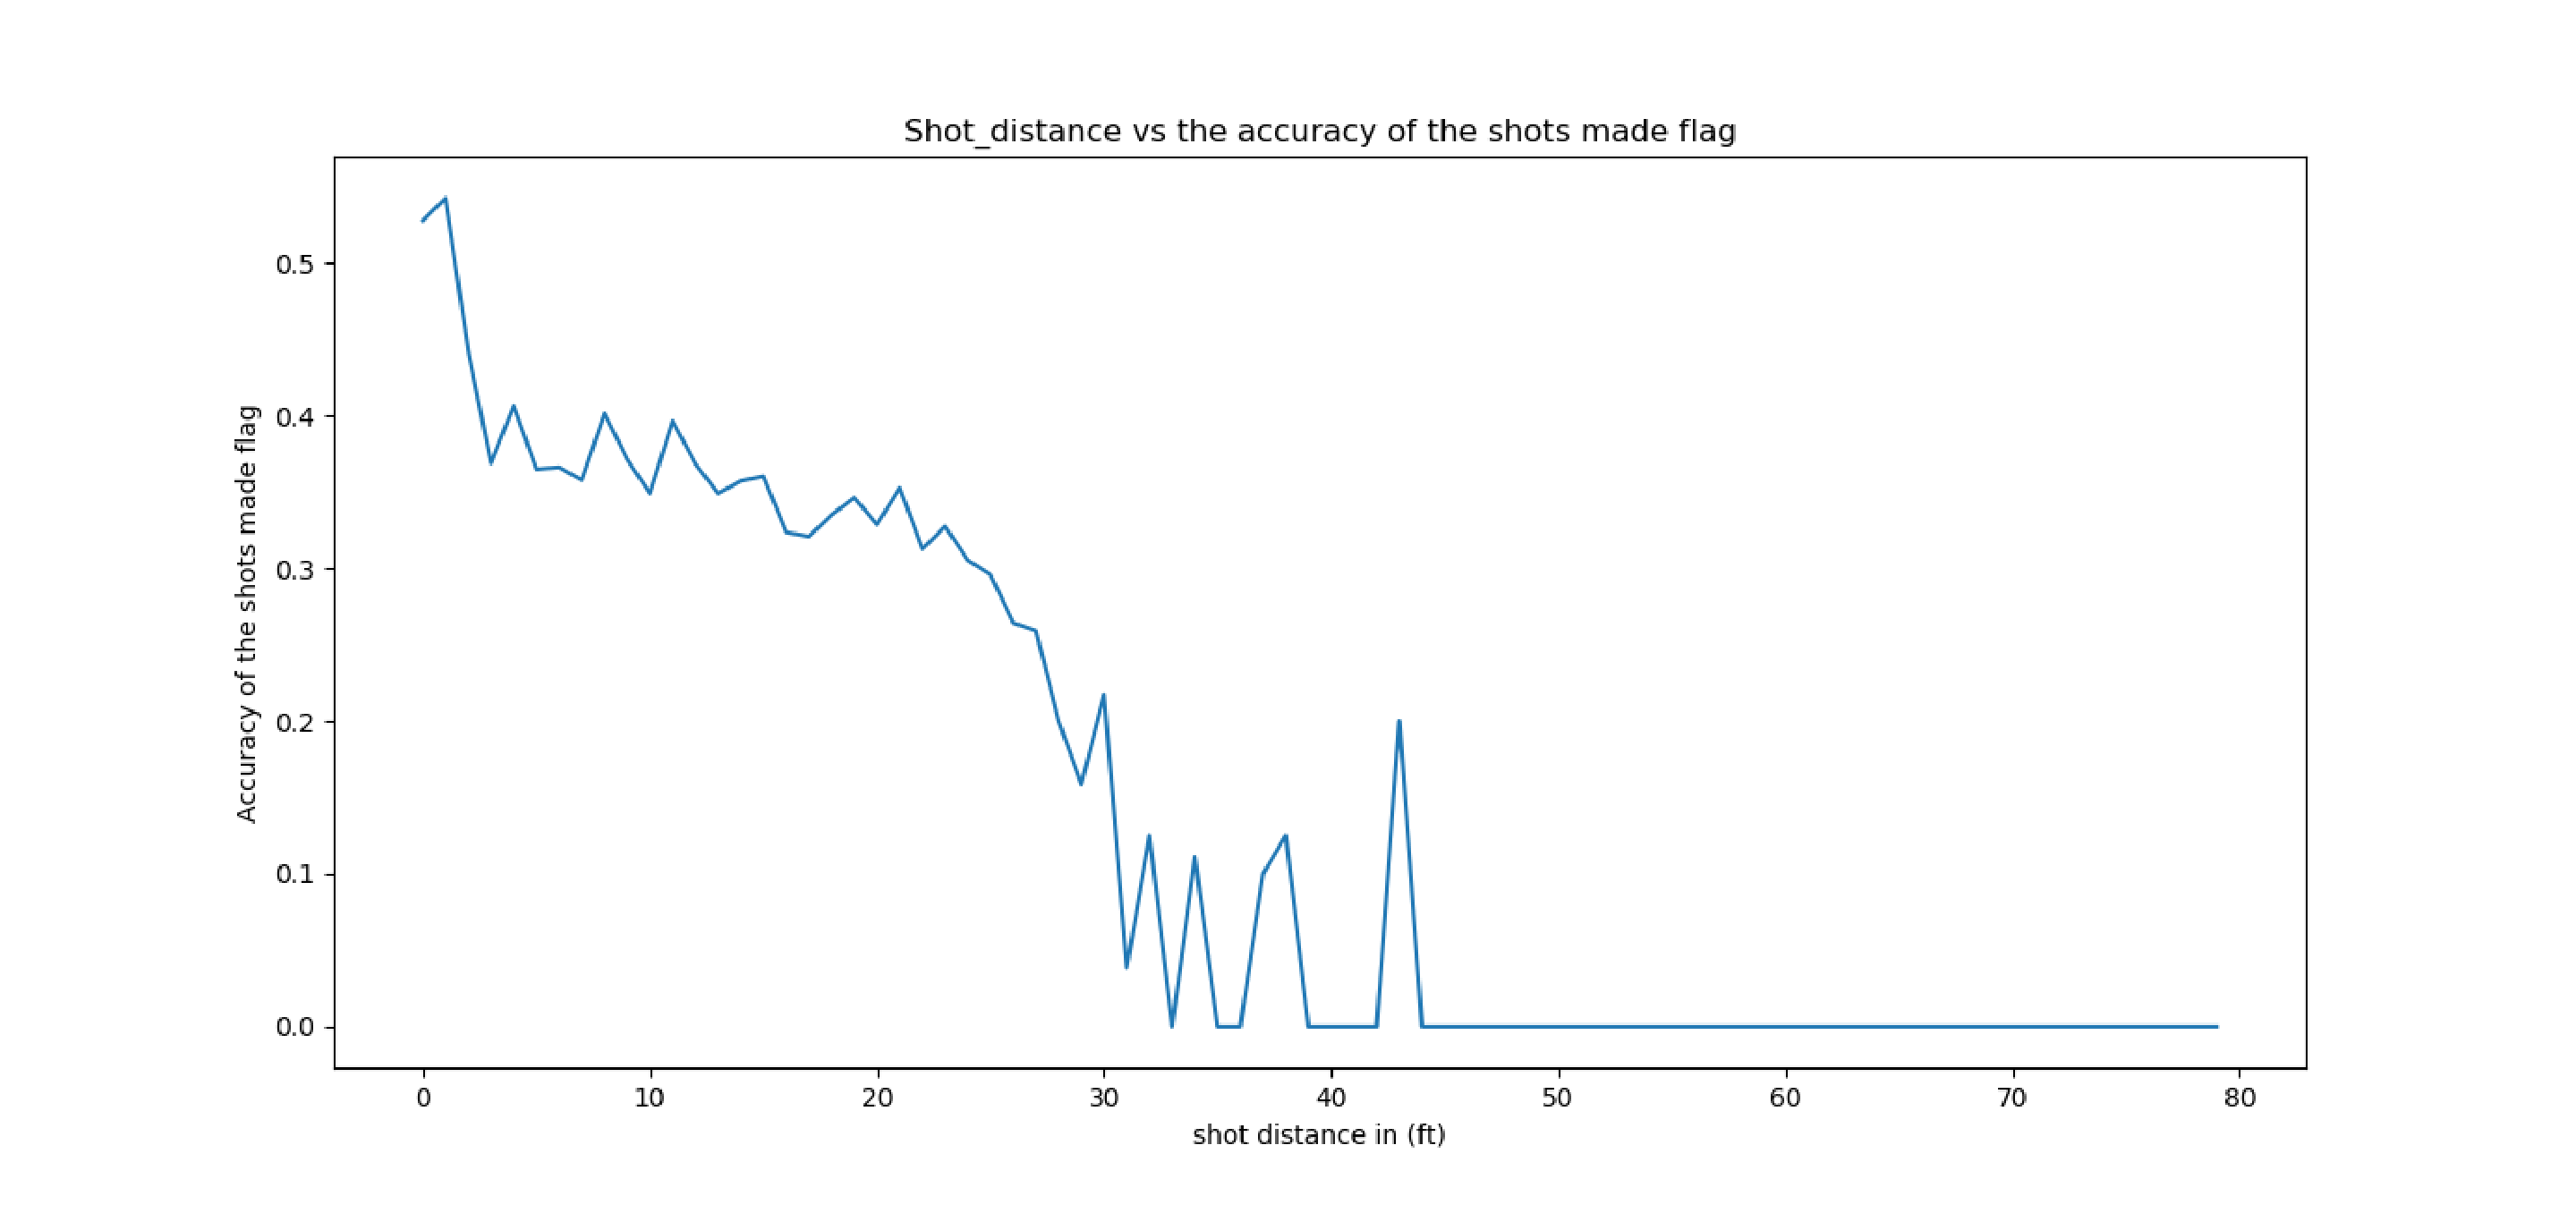
\includegraphics[width=.3\linewidth]{s.eps}
		\quad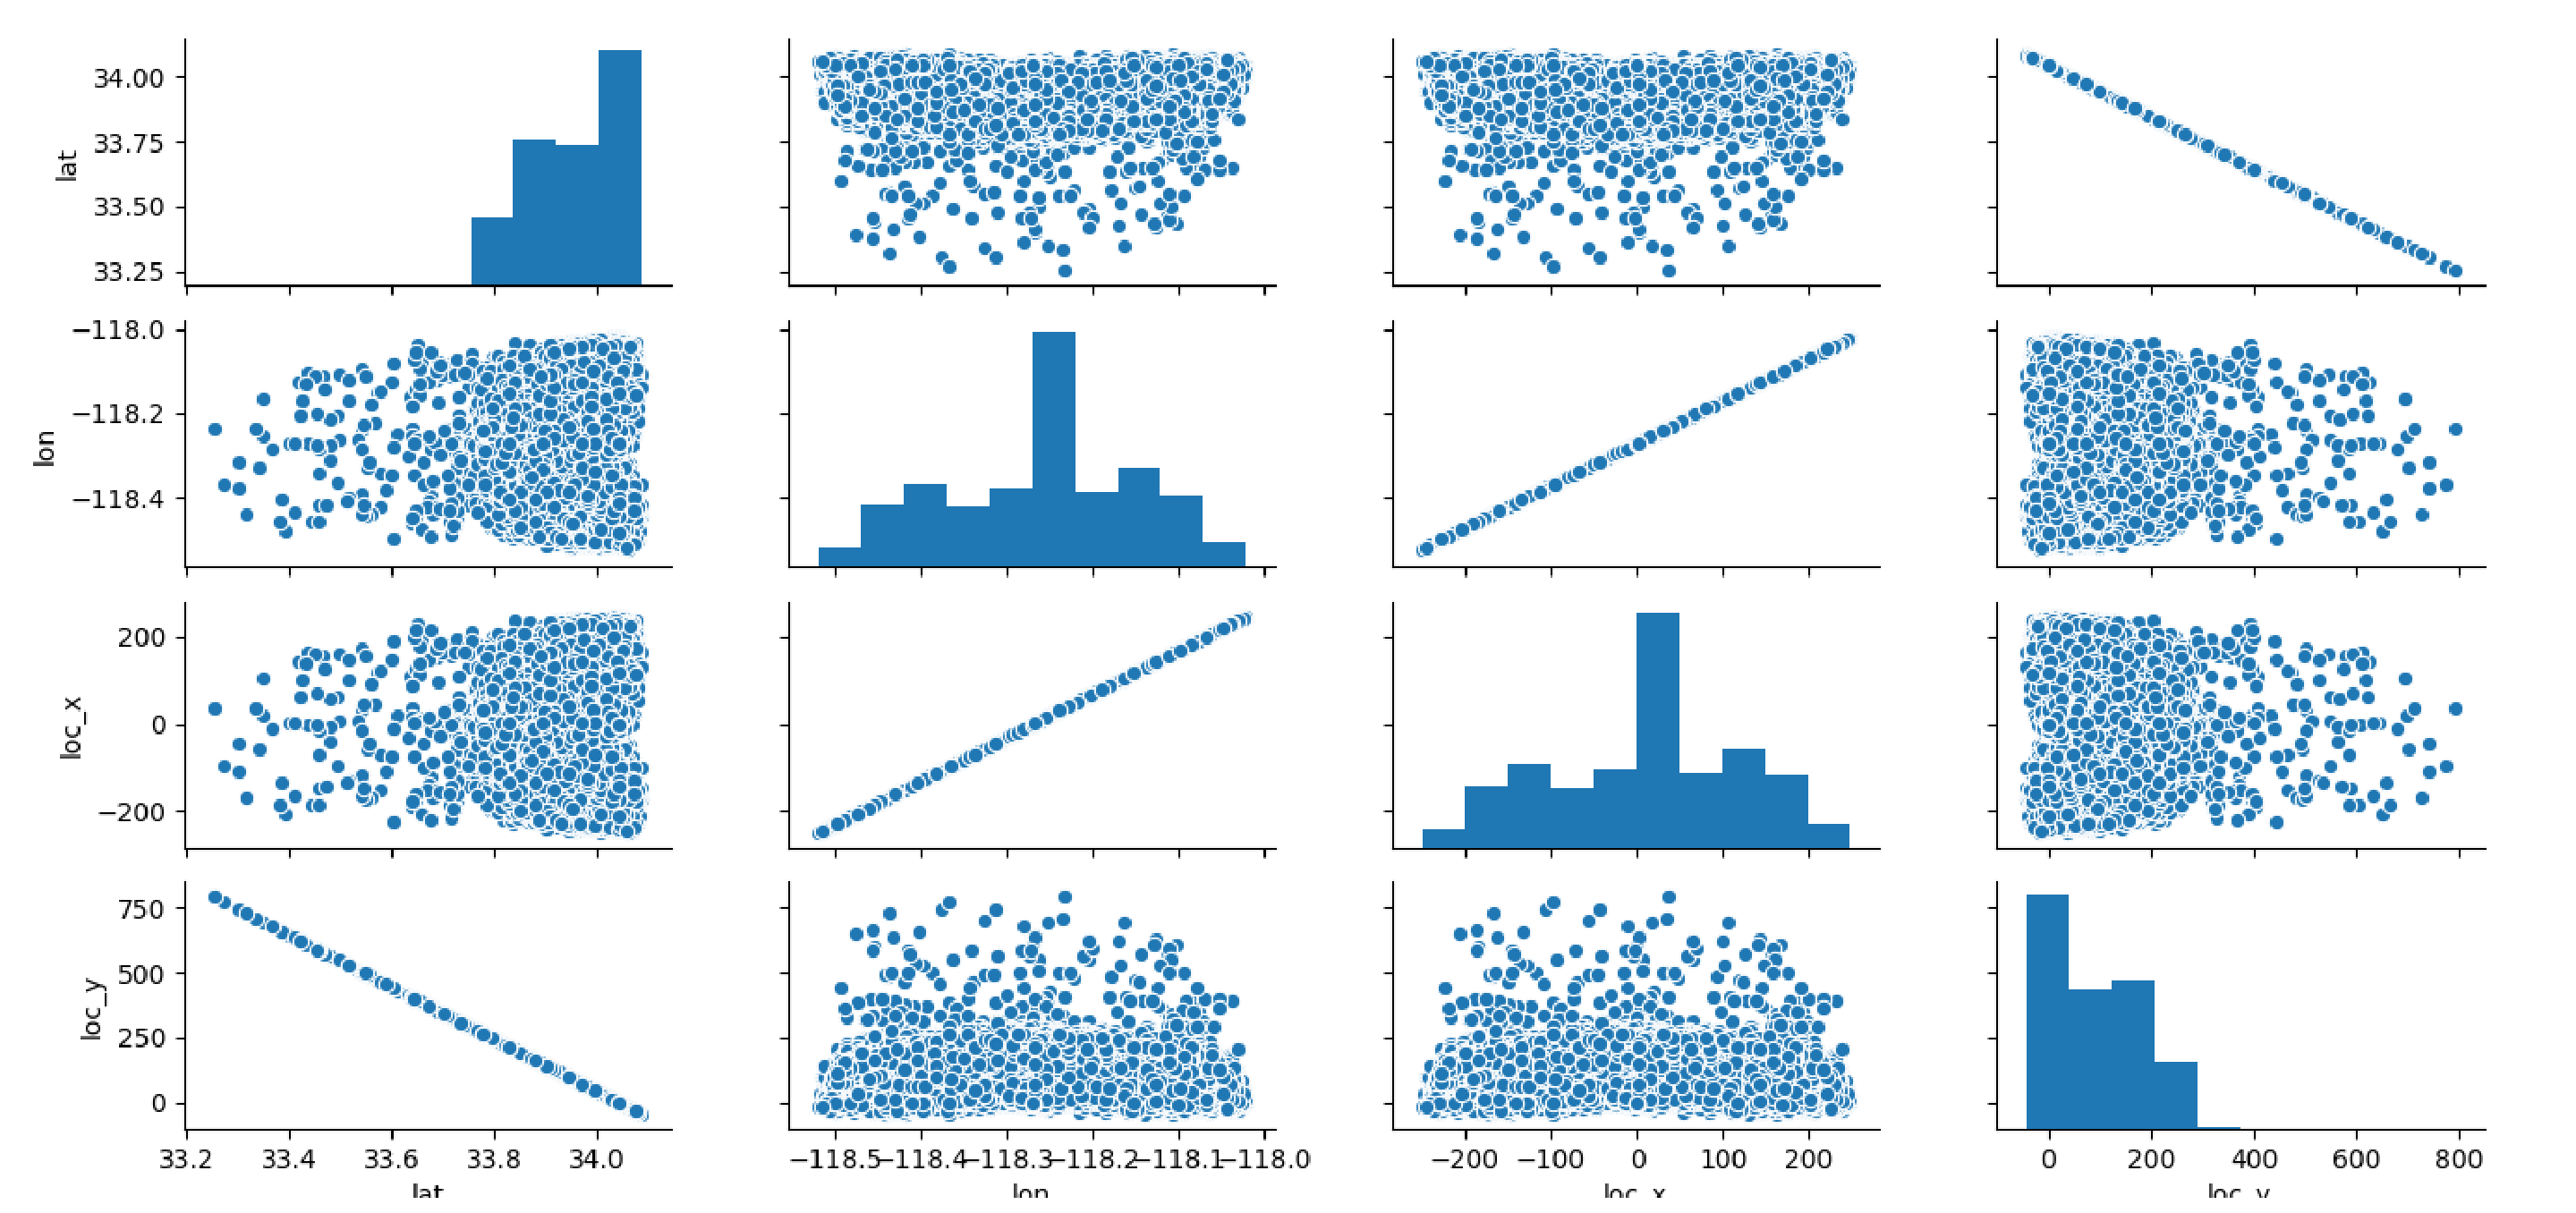
\includegraphics[width=.3\linewidth,height=.2\linewidth]{t.eps}	
	\end{center}
	\vspace{.3cm}
}
%%%%%%%%%% -------------------------------------------------------------------- %%%%%%%%%%


%%%%%%%%%% -------------------------------------------------------------------- %%%%%%%%%%

%\note{Note with default behavior}

%\note[targetoffsetx=12cm, targetoffsety=-1cm, angle=20, rotate=25]
%{Note \\ offset and rotated}

 % First column - second block


%%%%%%%%%% -------------------------------------------------------------------- %%%%%%%%%%
\block{Feature Engineering}{\item \textbf{Data Cleaning:} \newline
	Some of attributes show clusters: 
  	hair\_length and seconds\_remaining, 
  	hair\_length and bone\_length. 
  	So create new variable 
  	with multiplication of these columns: 

  	\begin{description}
  		row[total\_seconds] = row[seconds\_remaining]*row[minutes\_remaining] \newline
After that,we can remove the minutes and the seconds columns.
  	\end{description}


\item \textbf{Data Transformation:} \newline 
Categorical variables such as action\_type,combined\_shot\_type,season,shot\_type, 
shot\_zone\_range 
and opponent,we can create the dummy variables for further analysis.



}
%%%%%%%%%% -------------------------------------------------------------------- %%%%%%%%%%


% SECOND column
\column{0.5}
 %Second column with first block's top edge aligned with with previous column's top.

%%%%%%%%%% -------------------------------------------------------------------- %%%%%%%%%%
\block{Algorithm}{
	There are many machine learning algorithms 
	for classification problem. Choose the following algorithms, 
	use original train data and 
	new train data to train the models,
	and determine a set of optimal parameters 
	through Grid Search.

	\begin{itemize}
		\item RandomForest 
		\item LogisticRegression
		\item KNeighbors 
	\end{itemize}

}


%%%%%%%%%% -------------------------------------------------------------------- %%%%%%%%%%
\block[titleleft]{Forcast Result}
{
	The following are the best parameters and 
	the Best Score in training of 
	the base models 
	in original train data. 
	
	\item Best Parameters of Models
\begin{description}
	\item[RandomForest] 'criterion': 'entropy', 'max\_depth': 5, 
	'max\_features': None, 'n\_estimators': 100
	\item[LogisticRegression] 'C': 1, 'penalty': '11'
	\item[KNeighbors] 'algorithm': 'auto', 'leaf\_size': 10, 
	'n\_neighbors': 20, 'p': 5, 'weights': 'uniform'
	
\end{description}
	\vspace{.5cm}

\begin{itemize}
	\item Accuracy of these Models
\end{itemize}
\vspace{.5cm}
	\begin{center}

		\begin{tabular}{cccc}
	
			%\bottomrule
				\hline
			& RF  & LR  & KNN \\
				\hline
			Best Score & 0.638  & 0.682  & 0.568\\
				\hline
		\end{tabular}

	\end{center}

From the table,
it shows that the accuracy of 
each model is not much different.
and  it has shown that logistic regression runs better than others.
\newline
	
}
%%%%%%%%%% -------------------------------------------------------------------- %%%%%%%%%%


% Second column - second block
%%%%%%%%%% -------------------------------------------------------------------- %%%%%%%%%%
\block[titlewidthscale=1, bodywidthscale=1]
{Conclusion}
{
	\begin{description}
		\item[Exploratory Data Analysis] It is an 
		exploratory analysis of the data can 
		 
		provide the necessary conclusions 
		for data processing and modeling.
		\vspace{.5cm}
		\item[Data Preprocessing] This step contains
		dealing with missing data and outliers,
		changing categorical variable 
		into one-hot code and so on.
		\vspace{.5cm}
		\item[Feature Engineering] It's the 
		most important thing.
		Create as more as poosible features,
		then select the most useful features.
		\vspace{.5cm}
		\item[Model Training] The models have 
		many parameters,
		and can use Grid Search to find 
		the optimal paratemers.	
	\end{description}
}
%%%%%%%%%% -------------------------------------------------------------------- %%%%%%%%%%


% Bottomblock
%%%%%%%%%% -------------------------------------------------------------------- %%%%%%%%%%
\colorlet{notebgcolor}{blue!20}
\colorlet{notefrcolor}{blue!20}
\note[targetoffsetx=8cm, targetoffsety=-4cm, angle=30, rotate=15,
radius=2cm, width=.26\textwidth]{
Acknowledgement
\begin{itemize}
    \item
    Thanks!
 \end{itemize}
}

%\note[targetoffsetx=8cm, targetoffsety=-10cm,rotate=0,angle=180,radius=8cm,width=.46\textwidth,innersep=.1cm]{
%Acknowledgement
%}

%\block[titlewidthscale=0.9, bodywidthscale=0.9]
%{Acknowledgement}{
%}
%%%%%%%%%% -------------------------------------------------------------------- %%%%%%%%%%

\end{columns}


%%%%%%%%%% -------------------------------------------------------------------- %%%%%%%%%%
%[titleleft, titleoffsetx=2em, titleoffsety=1em, bodyoffsetx=2em,%
%roundedcorners=10, linewidth=0mm, titlewidthscale=0.7,%
%bodywidthscale=0.9, titlecenter]

%\colorlet{noteframecolor}{blue!20}
\colorlet{notebgcolor}{blue!20}
\colorlet{notefrcolor}{blue!20}
\note[targetoffsetx=-13cm, targetoffsety=-12cm,rotate=0,angle=180,radius=8cm,width=.96\textwidth,innersep=.4cm]
{
\begin{minipage}{0.3\linewidth}
\centering

\includegraphics[width=24cm]{logos/tulip-wordmark.eps}
\end{minipage}
\begin{minipage}{0.7\linewidth}
{ \centering
 Flip 00 project final report,
  27/10/2019, Nanjing, China
}
\end{minipage}
}
%%%%%%%%%% -------------------------------------------------------------------- %%%%%%%%%%


\end{document}

%\endinput
%%
%% End of file `tikzposter-template.tex'.
